\documentclass[a4paper]{esannV2}
\usepackage[dvips]{graphicx}
\usepackage[latin1]{inputenc}
\usepackage{amssymb,amsmath,array}
%***********************************************************************
% !!!! IMPORTANT NOTICE ON TEXT MARGINS !!!!!
%***********************************************************************
%
% Please avoid using DVI2PDF or PS2PDF converters: some undesired
% shifting/scaling may occur when using these programs
% It is strongly recommended to use the DVIPS converters, and to submit
% PS file. You may submit a PDF file if and only if you use ADOBE ACROBAT
% to convert your PS file to PDF.
%
% Check that you have set the paper size to A4 (and NOT to letter) in your
% dvi2ps converter, in Adobe Acrobat if you use it, and in any printer driver
% that you could use.  You also have to disable the 'scale to fit paper' option
% of your printer driver.
%
% In any case, please check carefully that the final size of the top and
% bottom margins is 5.2 cm and of the left and right margins is 4.4 cm.
% It is your responsibility to verify this important requirement.  If these margin requirements and not fulfilled at the end of your file generation process, please use the following commands to correct them.  Otherwise, please do not modify these commands.
%
\voffset 0 cm \hoffset 0 cm \addtolength{\textwidth}{0cm}
\addtolength{\textheight}{0cm}\addtolength{\leftmargin}{0cm}

\newcommand*{\IN}[0]{\ensuremath{\mathbb{N}}}

%\usepackage[english, status=draft]{fixme} % these 2 make fixme comments :) 
\usepackage[english]{fixme} % these 2 make fixme comments :) 
\fxusetheme{color}  

\usepackage{color}  % 25-11 added to highlight mautner changes
\usepackage{natbib} 
%bibstyle muss einer da sein, 
% setimmt wie der kram an \cite aussieht.
% https://de.wikibooks.org/wiki/LaTeX-W%C3%B6rterbuch:_bibliographystyle
%https://de.sharelatex.com/learn/Bibtex_bibliography_styles
%\bibliographystyle{abbrvnat} 
%\bibliographystyle{unsrt} 
%\bibliographystyle{plainnat}
                      %
%***********************************************************************
% !!!! USE OF THE esannV2 LaTeX STYLE FILE !!!!!
%***********************************************************************
%
% Some commands are inserted in the following .tex example file.  Therefore to
% set up your ESANN submission, please use this file and modify it to insert
% your text, rather than staring from a blank .tex file.  In this way, you will
% have the commands inserted in the right place.

\begin{document}
%style file for ESANN manuscripts
\title{Sampling graphs with long range dependencies}

%***********************************************************************
% AUTHORS INFORMATION AREA
%***********************************************************************
\author{Fabrizio Costa, Stefan Mautner, Rolf Backofen
%
% Optional short acknowledgment: remove next line if non-needed
%\thanks{This is an optional funding source acknowledgement.}
%
% DO NOT MODIFY THE FOLLOWING '\vspace' ARGUMENT
\vspace{.3cm}\\
%
% Addresses and institutions (remove "1- " in case of a single institution)
Albert-Ludwigs University Freiburg - Department of Computer Science\\
Freiburg, 79085 - Germany \\
%
}




  

%***********************************************************************
% END OF AUTHORS INFORMATION AREA
%***********************************************************************

\maketitle

\begin{abstract}
Machine learning constructive approaches offer a way to answer
`design' questions given some exemplar solutions.  In particular,
graph constructive methods are of interest in chemo- and bio-informatics
domains where the task is to synthesize novel molecules with a desired
bioactivity. Unfortunately RNA polymers exhibit complex dependencies between
their different constituent parts with bounds spanning the entire length of
the sequence. Since modeling long range dependencies is a difficult problem,
we propose an efficient solution, based on graph coarsening that builds on top
of a recent constructive approach and we show encouraging experimental results
on a RNA synthesis task.
\end{abstract}



\section{Introduction}

Constructive machine learning addresses the problem of automatically `design'
artifacts given a concept expressed as a representative set of examples. The
task becomes particularly challenging in a discrete setting when the solution
space is exponential and direct enumeration approaches become unfeasible, as
it is the case in the domain of graphs with discrete labels. In \cite{costa16}
the problem of generating elements of a structured domain was framed as the
equivalent problem of sampling from a corresponding underlying probability
distribution defined over a (learned) class of structures. 
\fxnote{Specifically $\Rightarrow$ their solution was ?} 
Specifically they
employ a context-sensitive grammar to accurately model complex dependencies
between different parts of an instance. The authors acknowledge that an
approach based exclusively on a grammar is not sufficient since the number of
proposed graphs grows exponentially with the number of production rules in the
grammar. To address the issue \cite{costa16} proposes to use a Metropolis
Hastings (MH) Markov Chain Monte Carlo (MCMC) method, where the problem of
sampling is reduced to the easier task of {\em simulation}. They use the
context sensitive graph grammar to inform the MH proposal distribution, but
also introduce a probability density estimator to define the MH acceptance
procedure. This allows to deal separately with local and global constraints:
the locally context-sensitive graph grammar is used for the local constraints
and the regularized statistical model is used for the global or long range
constraints. The two approaches complement each other: the grammar is a
flexible non-parametric approach that can model complex dependencies between
vertices that are within a short path distance from each other; the
statistical model, instead, can employ the bias derived from the particular
functional family (linear) and the type of regularization used (a penalty over
the $\ell_2$ norm of the parameters) to generalize long range dependencies to
similar cases. This approach is therefore adequate when the underlying concept
exhibit local dependencies that are more complex than long range ones.
Unfortunately in some application domains instances can exhibit complex long
range dependencies between their different constituent parts. This is the case
for RNA polymers, long sequences of atomic entities (nucleotides) that self
interact, establishing pairwise bounds that can typically span the entire
length of the sequence.

A different way to view the issue of long range dependencies is that of the
appropriate scale of representation. Certain application domains exhibit
natural encodings, i.e.\ instances are encoded as graphs where nodes represent
specific entities, such as nucleotides in the case of RNA sequences. However,
it is known that a more effective functional description of RNA polymers can
be obtained in terms of structural components such as {\em stems} \/(stretches
of consecutive paired nucleotides) and {\em loops} \/(stretches of consecutive
unpaired nucleotides). Under this view, dependencies that are local at the
coarser scales correspond to longer range dependencies at the original scale.

A constructive system suitable for these domains needs to be able to
adequately model complex long range dependencies and is more effective if it
operates at a convenient coarser scale rather than that of the individual
units. Here we tackle all these issues extending the approach presented in
\cite{costa16} with two key ideas: 1) we allow a user/domain defined graph
coarsening procedure, and 2) we allow domain specific optimization procedures
to ensure that generated instances are always viable.


\section{Method}

\cite{costa16} presented an approach to sample graphs from an empirical
probability distribution using a variant of the Metropolis Hastings (MH)
algorithm \citep{metropolis1953equation}. The MH approach decomposes the
transition probability of an underlying  Markov process in two factors, 1) the
proposal  and 2) the acceptance-rejection probability distributions. The
algorithm starts from a seed element and iteratively proposes new instances
that are stochastically accepted if they fit appropriate membership
requirements. The key element for an efficient MH design is building the
proposal distribution in such a way that the generated elements will not be
rejected too often. To do so Costa suggests to use a grammar and infer its
rules from the available data using grammatical inference techniques upgraded
to structured domains (i.e.\ domains where instances are naturally represented
as labeled graphs).

More precisely, a {\em graph grammar} \citep{rozenberg1999handbook} is a
finite set of productions; a production is a triple $S=(M,D,E)$ where $M$ is
the ``mother'' graph, $D$ is the ``daughter'' graph and $E$ is an embedding
mechanism. Given a ``host'' graph $H$, a production is applied as follows: 1)
identify one occurrence of $M$ as an isomorphic subgraph of $H$; 2) remove $M$
from $H$ and obtain $H^-$; 3) replace $M$ by an isomorphic copy of $D$; and
finally 4) use the embedding mechanism $E$ to attach $D$ to $H^-$.
\cite{costa16} introduced an efficient graph grammar based on the concept of
{\em distributional semantics}
\citep{harris1954distributional,harris1968mathematical} and on the {\em
substitutability principle} \citep{Clark:2007}. Two key notions are defined:
{\em internal core graphs}\/ and {\em interface graphs}. An internal core graph
(or {\em core}\/ for simplicity), denoted $C^v_R(G)$, is a neighborhood graph of
$G$ of radius $R$ rooted in $v$. An interface graph, denoted $I^v_{R,T}(G)$ is
the difference graph of two neighborhood graphs of $G$ with the same root in
$v$ and radius $R$ and $R+T$. The difference graph is the graph induced by
the difference of the two vertex sets. Intuitively an interface
corresponds to the ``external shell'' of a core with {\em thickness} $T$. This
shell represents the context available for the definition of a production
rule. The general concepts of mother and daughter graphs are specialized as
follows: given a production $S$, the mother graph $M$ and the daughter graph
$D$ are union graphs of an interface graph and a correspondent internal core
graph with the additional constraint that the interface graphs in the daughter
and mother graph must be identical (up to isomorphism); finally, the embedding
mechanism $E$ is given by the isomorphic bijection between the interface
graphs. In words, new elements are produced by {\em swapping inner cores}\/ in
identical contexts. In Fig.~\ref{allcips} (left) a production step is applied
to a molecular graph $G$. The core $C_{R}^v(G)$ (dark) is determined by
vertices at maximal distance $R$ ($R=0$ in the figure) from a chosen root
vertex $v$. The interface $I_{R,T}^v(G)$ with \emph{thickness} $T=2$ is in a
lighter shade. Given a new core-interface pair (CIP) with matching interface,
the substitution can take place to yield the replacement of a carbon with a
nitrogen atom. Note that this type of production rules can be inferred
efficiently (i.e.\ in linear complexity) from a representative set of graphs
(see \citep{costa16} for details).



\subsection{Method extension}

Two main issues arise when dealing with complex structures such as RNA
polymers, we call them 1) the {\em resolution}\/ and 2) the {\em viability}
problem. Replacing only few nodes at
each iteration can be inefficient when instances consist of several hundreds
of nodes. It is known that for RNAs a more effective description is obtained
considering larger structural components such as stems  and loops. As for the
second issue, it is known that the function of RNA polymers depends on their
global structure (i.e.\ the set of pairs of interacting nucleotides), which can
significantly change when even a single nucleotide is altered. To deal with
these issues we propose two enhancements to Costa's approach: 1) a
grammar coarsening procedure and 2) a constraint integration procedure.


\textbf{Grammar coarsening.} The idea is to allow users to specify 
a coarsening procedure in a simple way. We do so via the notion of {\em edge
contraction}\/:
an operation which removes an edge from a graph while simultaneously merging
the two vertices that it previously joined. In addition we allow the more
general 
\fxnote{"notion of"  is bloat } 
notion of {\em vertex contraction}, which removes the restriction that
the contraction must occur over vertices sharing an incident edge.
\fxnote{explaining the cid  might be too much detail}
Both
procedures are defined using a node attribute $cid \in \IN$ called 
{\em contraction-identifier}\/ and contracting all vertices that share the same $cid$. 
We propose to use the contraction operation as a flexible way to
transform a graph to its coarser version, $G \mapsto G'$. Cores and interfaces
can now be defined exploiting the contracted graph. Starting from a CIP on the
coarse graph, we define the core as the sub graph induced by the vertices of
the original graph that have been contracted to vertices of the core of radius
$R$ in the coarse graph, $C_R^v(G',G)$.  The new interface graph
$I_{R,B}^v(G',G)$ is defined as the Cartesian product of the graph induced by
the nodes adjacent to the core nodes in $G$ at maximal distance $B$ (the
thickness in the base graph) and the interface graph on the coarse graph. In
words, we require that both the interface at base level and at coarse level
match for a core swap to take place.
\fxnote{imo its "an rna"}
In Fig.~\ref{allcips}  we depict a RNA
polymer graph at nucleotide level (center) and its coarse version (right)
where the contraction was informed by the notion of structural components such
as stems, hairpin loops and multiloops. Note that a core at coarse
level (in dark) made only of one node, corresponds to multiple nodes at
base level. Moreover, while the interface at base level requires only the
presence of few nucleotides, these have to belong to a context defined at the
coarse level that can span a much larger fraction of the instance and can be
viewed as a global localization indicator.

\begin{figure}[ht]
      \centering
        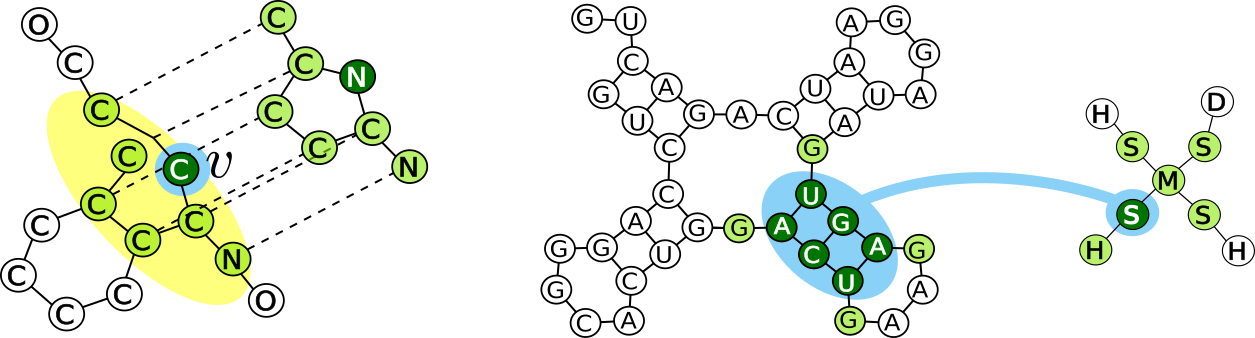
\includegraphics[width=0.7\linewidth]{images/allcipsinone.png}
      \caption{
      Core and interface subgraphs are marked in dark and light color
      respectively. Left: Molecular graph with indicated core substitution.
      Mid: RNA encoding with nucleotide level resolution.  Right:  
      RNA encoding with structural element resolution, with symbols: 
      H)airpin, M)ultiloop, S)tem, D)angling end.}
      \label{allcips}
\end{figure}


\textbf{Constraint integration.} It should be possible to easily make use of
specific feasibility constraints when these are available for a given domain.
For RNAs the relation between sequence and structure is known to be governed
by thermodynamical forces that seek to minimize the amount of free energy of
the molecule. The structure for a given sequence can be computed using
sophisticated dynamic programming optimization algorithms. To integrate these
constraints in the constructive protocol we let the user specify a
transformation function which maps candidate instances to feasible instances.
In our case the transformation takes a graph representing an RNA structure
constructed by the proposed procedure, removes the pairwise bounds and
recomputes them as the solution of a given folding algorithm. This
transformation ensures that we are computing the acceptance probability always
on viable RNA structures.


\section{Empirical evaluation and discussion}

RNA polymers cover essential biological roles ranging from coding, decoding,
regulation and expression of genes. The RFam database \citep{rfam} groups
known RNA sequences in functionally and evolutionarily related {\em families}. To
empirically investigate the performance of the proposed constructive approach
we selected the SAM-I/IV variant riboswitch (RF01725) and SAM riboswitch (S
box leader) (RF00162), which are families that exhibit a rich structure (e.g.
that do not consist only of a single hairpin). The general aim is to
synthesize functionally equivalent but novel sequences, a task with important
biomedical applications.


%\color{blue}
% here we describe how we obtain the secondary structure
The secondary structure of a sequence can not be reliably computed
using the sequence alone.
%\color{black} \color{red}
%When working with RNAs, the feasibility constraints are related to the
%structure determination. \color{black}
\fxnote{to improve accuracy $\rightarrow$ bloat}
To improve accuracy
we use a two step approach:
given a candidate sequence we 1) identify $k$ nearest neighbors among the
available training instances, then 2) we align the $k+1$ sequences using the
\emph{MUSCLE} (MUltiple Sequence Comparison by Log- Expectation) program
\citep{muscle} and compute the consensus structure using the \emph{RNAalifold}
program \citep{rnaalifold}. This procedure identifies
the most representative structure in the ensemble of possible suboptimal
solutions.

In order to evaluate if the constructed sequences are functionally equivalent
to the original examples, we use an independent state-of-the-art computational
\fxnote{is it 100\% clear that rfam is the oracle? }
approach as {\em oracle}\footnote{The correct, and expensive, procedure would
instead be to synthesize the sequences and test their functionality in a
biological experiment.}. To define the membership of a sequence to a given
family, the RFam database uses the covariance model computed by the program
\emph{Infernal} (INFERence of RNA ALignment) \citep{infernal} induced over a
hand curated set of representative sequences.
In Fig.~\ref{infeval} we report the average score achieved by the constructed
sequences as the training set increases.
\fxnote{training set \emph{size}?}
The black dotted horizontal line indicates
the family specific threshold above which the Infernal model accepts a
sequence as a valid instance of the family. In blue we report the results for
the proposed extension and in red the results for the original method.
%\color{blue}
Infernal can also learn covariance models and use these to generate new
sequences. The dashed line represents the performance of this approach.
To make the methods comparable, we trained the 
covariance model with consensus structures obtained 
by muscle and RNAalifold.
%To increase the quality of the output we used the parameter
%to exponentiate the probabilities in the model.
%\color{black}
We note that the proposed approach with the coarsening strategy consistently improves the quality of the results. 

In \cite{costa16}  \emph{the constructive learning problem for finite
samples} is formally specified as the optimization of a parametric generator
for two competing objectives: on the one hand one should obtain similar
probability density estimators when these are trained on the original data or
\fxnote{or $\rightarrow$ and ? i am not sure}
on the generated data; on the other hand the generated instances should be
different from those already known in the training phase\footnote{The notion
of similarity between probability density estimators is defined in terms of
Kullback-Leibler divergence and the notion of similarity between instances of
a structured domain is defined in terms of a set graph kernel, see
\citep{costa16} for details.}. In Fig.~\ref{learncurve} we evaluate these
properties as the training set increases. We observe that the similarity tends
to decrease as more diverse material becomes available and that also the
divergence tends to vanish, indicating that the instances generated induce the
same probability density as the original ones, albeit being increasingly
different.


\begin{figure}[ht]
      \centering
  \begin{minipage}[b]{0.47\textwidth}
    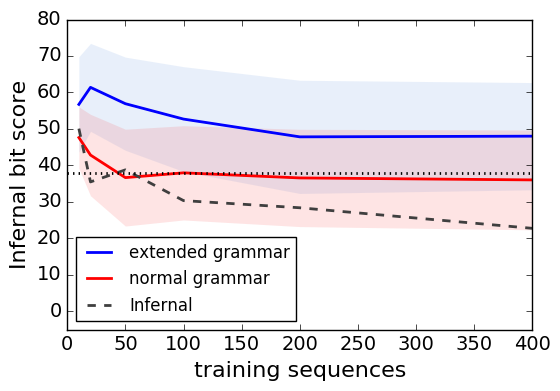
\includegraphics[width=\textwidth]{images/infernal.png}
      \caption{\footnotesize{Estimated equivalence by Infernal.}}
      \label{infeval}
  \end{minipage}
  \hfill \begin{minipage}[b]{0.51\textwidth}
    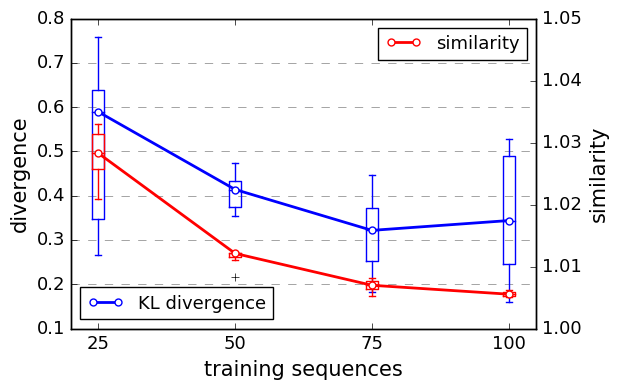
\includegraphics[width=\textwidth]{images/learningcurve.png}
      \caption{\footnotesize{Functional vs structural similarity.}}
     \label{learncurve}
  \end{minipage}
\end{figure}

    
 
\section{Conclusion}

We have introduced a generic approach to tackle the problem of long range
dependency modeling for a constructive machine learning approach.
Preliminary results are encouraging and show that we can propose novel
\fxnote{example sample $\rightarrow$ sample example ? }
RNA sequences that are functionally equivalent to an original example sample.
The coarsening procedure allows the injection of domain knowledge,
significantly improving the quality of the results over the original non domain
specific approach. 

In future work we will investigate how to learn task
specific coarsening schemes in a supervised fashion directly from data.



% ****************************************************************************
% BIBLIOGRAPHY AREA
% ****************************************************************************

\begin{footnotesize}

\bibliographystyle{unsrt}
\bibliography{mybib}

\end{footnotesize}

% ****************************************************************************
% END OF BIBLIOGRAPHY AREA
% ****************************************************************************

\end{document}
